In this section, we'll show you how we'll organize the implementation work of the web application. First, we'll decompose the implementation in several modules. Then, we'll organize it in a gantt diagram. \\

\subsection{Modules decomposition}
\begin{itemize}
\item a system kernel with object oriented model related with database, a base for pages display, utils functions
\item Connection/subscribing system
\item Search system
\item Account manager
\item Offer/Demand creator
\item Transaction aknowlegement
\item System related to organisations (user managing, offer/demand supervisor)
\item Group manager
\item E-mail and ID-cards validation
\end{itemize}

\subsection{Extensions}
In the previous report, we made the choice to implement an internal message service between the users to help to communicate while making transactions.There is a module in RoR which already implement this kind of service. We'll have to learn how to use it and put it into our application. \\

\subsection{Estimation and distribution of modules}
Since we choose a framework we didn't work with yet, it's difficult to know how much time will be needed to complete the first module (Kernel). After the development of this module, the others seems to have equivalent difficulty. It will be easier for us to share the work. We will not give now some specific modules to a specific group member. We will try to assign the modules in terms of each member qualifications.

\subsection{Gantt diagram}
\begin{figure}[!ht]
	\begin{center}
		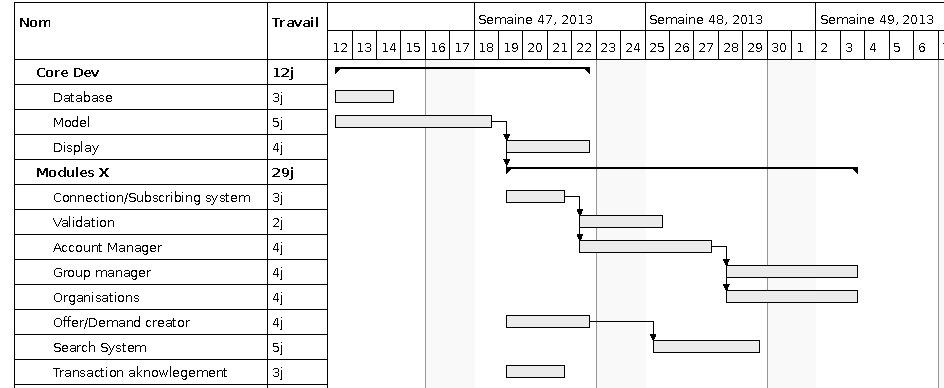
\includegraphics[width=\textwidth]{gantt_2_22_2_76.pdf}
		\caption{Gantt chart}
		\label{fig:gantt}
	\end{center}
\end{figure}